\begin{figure}[tb]
\centering
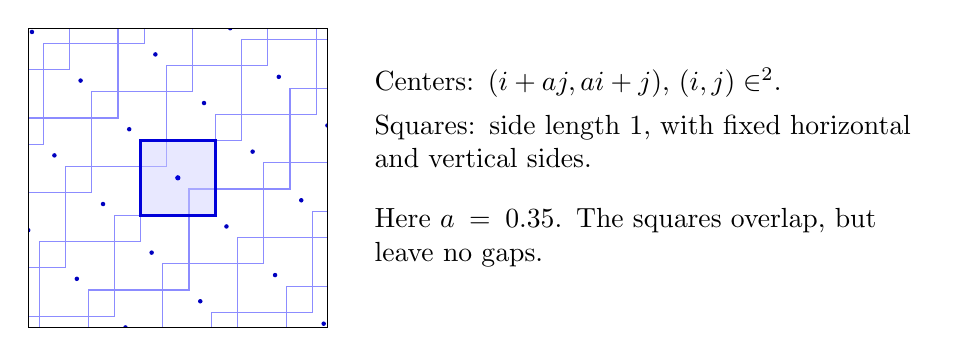
\begin{tikzpicture}[scale=0.95]
 \begin{scope}
  \clip (-2,-2) rectangle (2,2);
  \foreach \i in {-4,...,4} {\foreach \j in {-4,...,4} {
   \pgfmathsetmacro{\cx}{\i+.35*\j}
   \pgfmathsetmacro{\cy}{\j+.35*\i}
   \draw[blue!45,line width=.4pt]
     ({\cx-.5},{\cy-.5}) rectangle ({\cx+.5},{\cy+.5});
   \fill[blue!75!black] (\cx,\cy) circle (.03);
  }}
  \fill[blue!20,opacity=.45] (-.5,-.5) rectangle (.5,.5);
  \draw[blue!85!black,line width=1.1pt] (-.5,-.5) rectangle (.5,.5);
  \fill[blue!85!black] (0,0) circle (.035);
 \end{scope}
 \draw (-2,-2) rectangle (2,2);
 \node[align=left,anchor=west,text width=7cm] at (2.5,.8)
   {Centers: $(i+aj,ai+j)$, $(i,j)\in\Z^2$.\\[4pt]
    Squares: side length $1$, with fixed horizontal and vertical sides.};
 \node[align=left,anchor=west,text width=7cm] at (2.5,-.8)
   {Here $a=0.35$. The squares overlap, but leave no gaps.};
\end{tikzpicture}
\caption{A bounded window in the lattice covering of
Lemma~\ref{b:lattice}, with the square at the origin highlighted.
The squares keep their original shape and orientation as their centers move.
The affine construction uses an orthonormal basis for each frozen
differential. Its finite approximation retains fine-grid centers only
near the corresponding coarse label square.}
\label{b:figure-lattice}
\end{figure}
